\documentclass{VUMIFPSkursinis}
\usepackage{algorithmicx}
\usepackage{algorithm}
\usepackage{algpseudocode}
\usepackage{amsfonts}
\usepackage{amsmath}
\usepackage{bm}
\usepackage{caption}
\usepackage{color}
\usepackage{float}
\usepackage{graphicx}
\usepackage{listings}
\usepackage{subfig}
\usepackage{array}
\usepackage{wrapfig}
\usepackage{tabu}

% Titulinio aprašas
\university{Vilniaus universitetas}
\faculty{Matematikos ir informatikos fakultetas}
\department{Programų sistemų katedra}
\papertype{Kursinis darbas}
\title{Blokų grandinių duomenų bazės finansinių duomenų kaupimui}
\titleineng{Blockchain Databases for Financial Data}
\status{4 kurso 3 grupės studentas}
\author{Matas Savickis}
% \secondauthor{Vardonis Pavardonis} % Pridėti antrą autorių
\supervisor{dr. Vytautas Valaitis}
\date{Vilnius – \the\year}

% Nustatymai
% \setmainfont{Palemonas} % Pakeisti teksto šriftą į Palemonas (turi būti įdiegtas sistemoje)
\bibliography{bibliografija}

\begin{document}

\maketitle
\thispagestyle{empty} 

\tableofcontents

\sectionnonum{Padėka}
Noriu padėkoti savo darbo vadovui daktarui Vytautui Valaičiui už pagalbą, vadovavimą ir skirtą savo laisvą vasaros laiką padedant man rašyti šį darbą.
\pagebreak

\sectionnonum{Įvadas}
\setcounter{page}{1}
\thispagestyle{empty} 
Per pastaruosius keletą metų blokų grandinių technologija susilaukė didelio žmonių susidomėjimo. 
Šis susidomėjimas daugiausiai kilo dėl išpopulerėjusių kriptovaliutų, tokių kaip Bitcoin, Etherium, Litecoin ir daugeliu kitų 
kurios ir yra paremtos blokų grandinių technologija. Šią technologiją 2008 metais sukūrė Satošis Nakamoto \cite{BlockChain}. 
2009 metais Nakamoto realizavo blokų grandinių technologiją sukurdamas Bitcoin kriptovaliutą \cite{Bitcoin}. 
Nors, šiuo metu, žmonių susidomėjimas kripto valiutomis ir yra sumažėjęs \cite{Trends}, tačiau informacinių technologijų industrija 
mato daugiau blokų grandinių panaudojimo atveju negu tik kriptovaliutos. Vienas iš blokų grandinių panaudojimo atvejų yra 
blokų grandinių duomenų bazės. Reliacinės ir dokumentų duomenų bazės ilgą laiką buvo pagrindinis duomenų saugojimo būdas. 
Tačiau šios duomenų bazės turi ir savo trūkumų, saugant duomenis reliacinėse duomenų bazėse kyla duomenų integralumo problemos \cite{Integrity}. Naudojant duomenų bazes finansinėms transakcijoms sekti kyla dvigubo pinigų išleidimo problema\cite{Double}. Naudojantis tradicinėmis duomenų bazėmis 
taip pat kyla pasitikėjimo problema, visa duomenų prieiga yra trečiosios šalies valdžioje, ir vartotojas turi pasitikėti, kad duomenys nebus pakeisti be jo žinios.
Per pastaruosius kelis metus šias problemas
buvo stengtasi išspręsti kuriant duomenų bazes paremtas blokų grandinių technologija. Privačios blokų grandinių duomenų bazės užtikrina pasitikėjimą, nes kiekvienas vartotojas turi visą duomenų 
bazės kopiją. Darant pakeitimus tokioje duomenų bazėje kiekvienas vartotojas turi sutikti su daromais pakeitimais ir saugo visų pakeitimų istoriją. Blokų grandinių duomenų bazės išsprendžia duomenų integralumo ir
dvigubo pinigų išleidimo problemą, nes kiekvienas mazgas blokų grandinės tinkle gali palyginti savo turimus duomenis su kitais mazgais. 
Nors blokų grandinės išsprendžia išvardytas problemas, tačiau finansiniams duomenims taip pat svarbu greitis, duomenų pasiekiamumas ir sistemos galimybė išlikti funkcionaliai po tam tikrų trikdžių. 
Yra nemaža aibė blokinių grandinių duomenų bazių(R3 Corda, BigChain DB), bei didelis pasirinkimas NoSQL duomenų bazių(Mongo DB, Redis, Neo4j) tačiau šiam darbui buvo pasirinktos
Hyperledger Fabric ir Apache Cassandra, nes šios duomenų bazės yra naudojamos finansiniams duomenims saugoti \cite{BnkH,BnkC}.

\sectionnonum{Tikslas}

CAP teorema - teorema sakanti, kad paskirstytoje duomenų sistemoje neįmanoma užtikrinti daugiau dviejų punktų: Duomenų neprieštaringumas, duomenų pasiekiamumas, dalivijusi toleravimas. \newline
Šio darbo tikslas yra:
\begin{itemize}
\item{Palyginti Apache Cassandra ir Hyperledger Fabric pagal išskirtas metrikas.}
\item{Palyginti Apache Cassandra ir Hyperledger Fabric pagal CAP teoremą.}
\end{itemize}

\sectionnonum{Uždaviniai}
\begin{enumerate}
\item{Išskirti bendras metrikas, pagal kurias būtų galima palyginti Apache Cassandra ir Hyperledger Fabric duomenų bazes.}
\item{Palyginti Apache Cassandra ir Hyperledger Fabric pagal išskirtas metrikas.}
\item{Išskirti esamų tyrimų trūkumus ir galimas sritis ateities darbams.}
\item{Palyginti Apache Cassandra su Hyperledger Fabric pagal CAP teoremos punktus.}
\end{enumerate}
\pagebreak
\section{Duomenų bazių greičių tyrimų literatūros analizė}

\subsection{Metrikos}
Šiame skyriuje bus apžvelgiami tyrimai, kuriuose buvo analizuotas ir vertintas Hyperledger Fabric \cite{IMBResearch,ThailandPerf,ShaFabPerf} ir Apache Cassandra \cite{BITCass,MonCas} veikimas. 
Šiuose darbuose buvo vertinamas: transakcijų praeinamumas, transakcijų vėlavimas, procesoriaus resursų sunaudojimas, mazgų skaičius paskirstytoje duomenų bazėje. \newline
Šiame darbe Hyperledger Fabric ir Apache Cassandra bus lyginama pagal:
\begin{itemize}
\item{Transakcijų praeinamumas - kiek transakcijų duomenų bazė gali apdoroti per sekundę.}
\item{Vėlavimas - kiek laiko užtrunka nuo transakcijos išsiuntimo iki jos patvirtinimo duomenų bazėje.}
\end{itemize}

\subsection{Hyperledger Fabric}
Hyperleadger yra atviro kodo blokų grandinės pradėtos kurti Linux fondo. Šio projekto tikslas yra gerinti tarp industrinį bendradarbiavimą kuriant blokų grandines kurios užtikrintų 
patikimą, greitą ir saugų finansinių duomenų perdavimą pagrindinėse technologijų, finansų ir produktų tiekimo kompanijose \cite{LinuxHyper}. Šiame skirsnyje bus apžvelgti 
Hyperledger Fabric, populiariausios Hyperledger realizacijos, architektūra, greičio tyrimai, kaip šie tyrimai buvo atlikti, kokie parametrai įtakoja Hyperledger greitį ir pateikta tolimesnės analizės pasiūlymai. 
\subsubsection{Architektūra}
Hyperledger Fabric(toliau - Fabric) yra privati blokų grandinė skirta įmonių lygio aplikacijoms. 
Ši blokų grandinė gali vykdyti arbitrišką išmanujį kontraktą parašyta Java, Go arba NodeJS kalbomis (grandinės kodai).
Fabric sudaro šios esybės:
\begin{itemize}
\item{Lygiarangis - šis mazgas yra atsakingas už grandinės kodą kurį vykdant yra įgyvendinamas išmanusis kontraktas. 
Lygiarangis savyje turi visą tinklo informaciją(angl. Ledger). }
\item{Rykiavimo servisas (angl. Ordering Service) - Rikiavimo serviso mazgas dalyvauja susitarimo(angl. consensus) 
protokole ir padalina bloką taip, kad jį būtų galima naudoti transakcijoms. Padalintas blokas būna persiunčiamas kitiems lygiarangiams.}
\item{Klientas - atsakingas už transakcijos siūlymo sukūrimą, ir išsiuntimą tinklo lygiarangiams. Gavus patvirtinimą iš lygiarangių vartotojas siunčia prašymą tvarkytojui, kad jis informaciją įtrauktų į bloką ir išsiūtu ją visiems tinklo perams.}
\end{itemize}
\subsubsection{Tranzakcijų valdymas}
Tranzakcijos vyksta trejomis fazėmis(1 pav.):
\begin{enumerate}
\item{Patvirtinimo fazė - simuliuojama transakcija su pasirinktais vienarangiais ir renkami būsenos pokyčiai.}
\item{Užsakymo fazė - užsakomos transakcijos per susitarimo protokolą.}
\item{Patvirtinimo fazė - patvirtinimas ir informacijos įdėjimas į didžiąją knygą.}
\end{enumerate}

\begin{figure}[H]
\centering
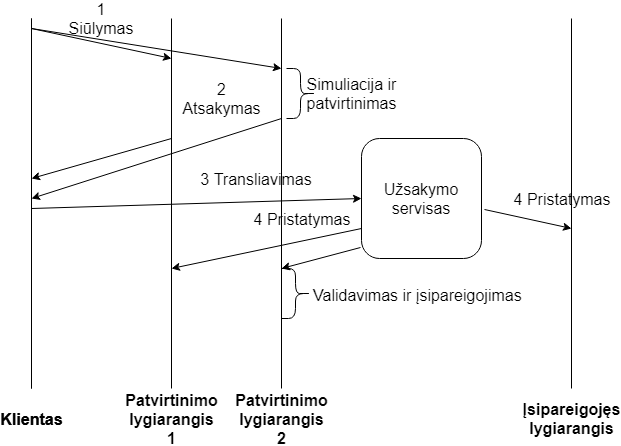
\includegraphics[scale=0.5]{img/MLP}
\caption{Transakcijų sekų diagrama} % Antraštė įterpiama po paveikslėlio
\label{img:mlp}
\end{figure}
\subsubsection{Parametrai}
Yra grupė parametrų \cite{IMBResearch} kurie įtakoja Fabric greitį 
\begin{itemize}
\item{Mazgų skaičius - vartotojų skaičius privačioje blokų grandinėje.}
\item{Transakcijų skaičius - keičiant transakcijų skaičių keičiasi vėlavimas ir pralaidumas.}
\item{Bloko dydis - transakcijos yra sugrupuojamos į blokus. Blokai yra siunčiami visiems tinklo vienarangiams. Užsakymo parašas 
būna verifikuojamas kiekvienam blokui, o perdavimo patvirtinimo parašas verifikuojamas kiekvienai transakcijai, todėl keičiant bloko dydį atsiranda kompromisas tarp palaidumo ir vėlavimo.}
\item{Patvirtinimo politika - diktuoja kiek transakcijų ir pasirašymų turi būti įvykdyta prieš siunčiant transakcijas užsakytoją. Didinant politikos sudėtingumą didės resursų sunaudojimas ir įvertinimo laikas.}
\item{Kanalai - izoliuoja transakcijas viena nuo kitos ir norint persiųsti transakcijas iš vieno kanalo į kitą turi būti patvirtintos, surikiuotos ir apdorotos nepriklausomai viena nuo kitos.}
\item{Resursų paskirstymas - kiekvienas lygiarangis vykdo grandinės kodą skirtą parašo skaičiavimams ir verifikavimo rutinoms. Keičiant procesoriaus branduolių skaičių keičiasi vykdymo greitis.}
\item{Būsenos duomenų bazė - Fabric naudoją dvi duomenų bazes, CouchDB ir GoLevelDB, kuriuose galima saugoti didžiosios knygos būseną.}
\end{itemize}
\subsubsection{Testavimo metodologija}
Šiame darbe apžvelgta trijų straipsnių duomenys, kuriuose naudota tokia kompiuterinė įranga:
\begin{center}
\begin{tabular}{ | m{5em} | m{10cm}| } 
\hline
\cite{IMBResearch}& x86 64 virtuali mašina IBM SoftLayer duomenų centre. 
Kiekvienai virtualiai mašinai yra suteikta 32 vCPUs Intel(R) Xeon(R)
CPU E5-2683 v3 @ 2.00GHz ir 32 GB atminties. Trys kliento mašinos skirtos generuoti apkrovą buvo paskirta
56 vCPU ir 128 GB RAM. Mazgai prijungti prie 3 Gbps duomenų centro tinklo \\ 
\hline
\cite{ThailandPerf}& Amazon AWS EC2
su Intel E5-1650 8 branduolių CPU,
15GB RAM, 128GB SSD \\ 
\hline
\cite{ShaFabPerf}& HPC serveris
su Intel(R) Xeon(R) CPU E5-2690, 2.60 GHz, 24 branduoliai
CPU, 64 GB RAM, Ubuntu 16.04 \\ 
\hline
\end{tabular}
\end{center}

\subsubsection{Tyrimų rezultatai}
\begin{figure}[H]
\centering
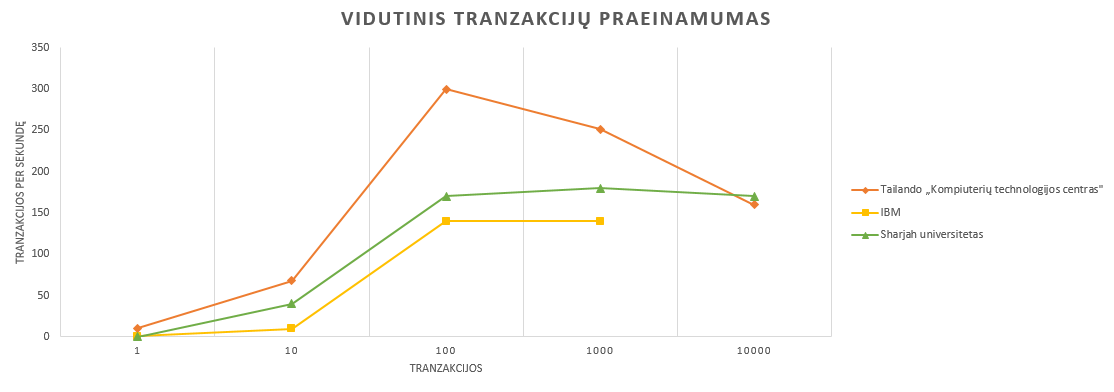
\includegraphics[scale=0.6]{img/Praein}
\caption{Transakcijų praeinamumas} % Antraštė įterpiama po paveikslėlio
\label{img:mlp}
\end{figure} 
\begin{figure}[H]
\centering
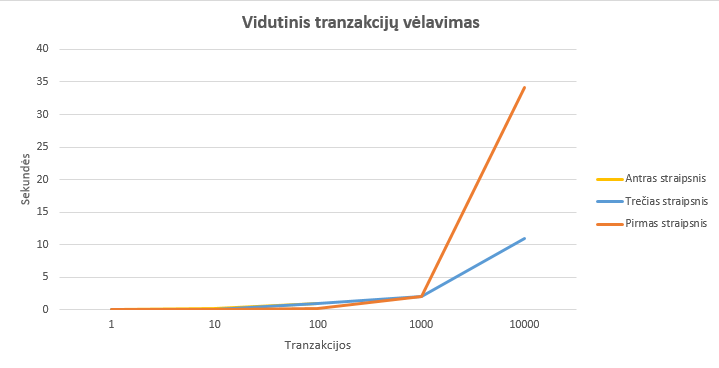
\includegraphics[scale=0.6]{img/Velav}
\caption{Transakcijų vėlavimas} % Antraštė įterpiama po paveikslėlio
\label{img:mlp}
\end{figure} 
\subsubsection{IBM tyrimo rezultatai}
IBM atliktame tyrime \cite{IMBResearch} buvo tiriama kaip keičiant Fabric parametrus keičiasi transakcijų praeinamumas ir vėlavimas. Didinant transakcijų atvykimo kiekį nuo 20 transakcijų per sekundę iki 100 praeinamumas didėja tiesiškai, o nuo 100 transakcijų per sekundę praeinamumas sustojo ir nebekilo. Bloko dydis praeinamumui įtakos neturėjo. 
\newline
Mažiausias vėlavimas būna pasirinkus mažiausia bloko dydį. Keičiant transakcijų atvykimo kiekį nuo 25 iki 125 vėlavimas išlieka apie 0,3 sekundės ir tuomet smarkiai kyla iki 10 sekundžių transakcijų 
atvykimo kiekį pakėlus iki 150 transakcijų. 
\newline
Iš šio tyrimo imsime geriausius rezultatus(2 pav. ir 3 pav.) ir vėliau lyginsime juos su Apache Cassandra duomenų baze. 
\subsubsection{Tailando ,,Kompiuterių technologijos centro" tyrimo rezultatai}
Tailando ,,Kompiuterių technologijos centro" atliktame darbe \cite{ThailandPerf} buvo simuliuojamos pinigų siuntimas, pinigų išdavimas ir vartotojų sukūrimas. Keliant transakcijų skaičių iki 100 praeinamumas kilo iki 299.85 transakcijų per sekundę. Didinant transakcijų skaičių iki 1000 praeinamumas pakito nežymiai, kaip ir IBM \cite{IMBResearch} atliktame darbe, ir didinant transakcijų skaičių iki 10000 praeinamumas krito iki 159.76 transakcijų per sekundę. 
Didinant transakcijas nuo 1 iki 100 vėlavimas kilo nežymiai, nuo 0.09 iki 0.17. Padidinus tranzakcijas nuo 100 iki 10000 staiga pakilo vėlavimas net iki 34.08 sekundžių.
\subsubsection{Sharjah universiteto tyrimo rezultatai}
Sharjah universiteto mokslininkų tyrime \cite{ShaFabPerf} Fabric 0.6 ir Fabric 1.0 transakcijų praeinamumas ir vėlavimas. Nuo 10 iki 100 transakcijų praeinamumas kilo nuo 40 transakcijų per sekundę iki 165 transakcijų per sekundę, toliau didinant transakcijų skaičių praeinamumas nebekito. Toks rezultatas gautas naudojant Fabric 1.0 versija ir praeinamumas geresnis negu Fabric 0.6 versijos. 
Didinant transakcijų skaičių nuo 10 iki 1000 vėlavimas pakilo nežymiai, nuo 0.1 sekundės iki 1 sekundės, tačiau padidinus transakcijų skaičių iki 10000 pastebėtas didelis vėlavimo pašokimas iki 10 sekundžių. Šio darbo metodologija buvo paremta jau minėtu Tailando mokslininkų darbu \cite{ThailandPerf}
\subsubsection{Tyrimų rezultatų apibendrinimas}
Iš aukščiau aptartų darbų(\cite{IMBResearch,ThailandPerf,ShaFabPerf}) pastebima tendencija, kad didinant transakcijų skaičių iki 100 praeinamumas kilo tiesiškai, o didinant transakcijų skaičių toliau praeinamumas nebekilo arba net krito(\cite{ThailandPerf}).
\newline
Didinant transakcijas nuo 1 iki 1000 vėlavimas praktiškai nekyla, ir tada nuo 1000 iki 10000 vėlavimas smarkiai šoktelėja. 
\subsection{Apache Cassandra}
Apache Cassandra yra atviro kodo, paskirstyta NoSQL duomenų bazė kuri palaiko klasterizavimą bei asinchroninį be valdančiojo kompiuterio duomenų replikavimą. Šios Cassandra galimybės yra panašios į blokinių grandinių duomenų bazių galimybes, todėl šiame skyriuje apžvelgsime jau padarytus 
Cassandra duomenų bazės našumo tyrimus. 

\subsubsection{Architektūra}
Apache Cassandra yra atviro kodo tarpusavio paskirstytoji duomenų bazė. Cassandra laikosi tarpusavio paskirstymo modelio. Laikantis šio modelio kiekvienas tinklo mazgas turi tą pačią struktūrą kas palengvina Cassandra praplėtimą. 
\linebreak
Cassandra duomenų struktūrą sudaro: 
\begin{itemize}
\item{Stulpelis - jį sudaro pavadinimas ir reikšmė.}
\item{Laiko žyma - rodanti kada paskutinį kartą stulpelis buvo pakeistas.}
\item{Eilės raktas - unikalus eilės identifikatorius.}
\item{Eilių šeima - vieta kurioje yra panašių stulpelių aibės.}
\item{Raktų erdvė - atitikmuo duomenų bazei reliacinėse duomenų bazėse.}
\end{itemize}
\begin{figure}[H]
\centering
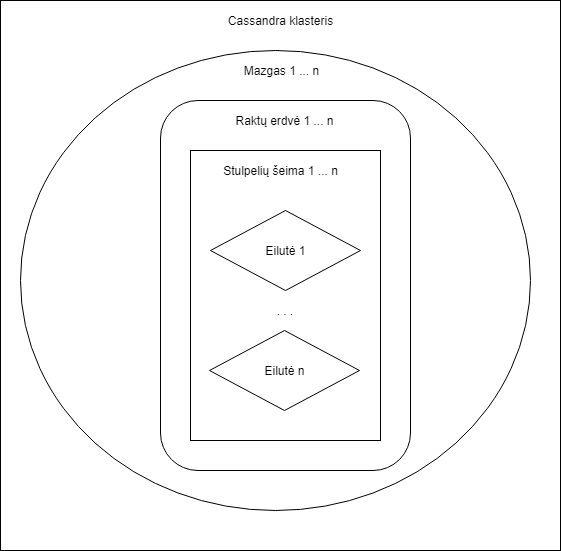
\includegraphics[scale=0.5]{img/CasArch}
\caption{Tranzakcijų vėlavimas} % Antraštė įterpiama po paveikslėlio
\label{img:mlp}
\end{figure}

` Replikavimas - darant užklausas galima pasirinkti replikavimo faktorių. Replikavimo faktorius nurodo per kiek klasterio mazgų užklausos duomenys bus kopijuojami. Didesnis replikavimo reiškia, kad duomenys klasteryje bus lengviau pasiekiami. Turint duomenis tik viename mazge ir praradus ryšį su tuo mazgu duomenys tinkle dings. Tačiau nustačius aukšta replikavimo faktorių Cassandra užtrunka daugiau laiko koordinuoti duomenis tinkle. 
\par
Skaidymas - nusako kaip duomenys bus paskirstyti mazguose. Šis funkcionalumas leidžia nurodyti kaip eilių raktai bus saugomi kas įtakoja kaip bus atliekamos užklausos į duomenų bazę.
\par
Paskalos - Cassandra naudoja ,,paskalų" protokolą kurio pagalba visi tinklo mazgai žino informaciją apie kitus tinklo mazgus. Mazgai seka informacija apie tai ar su kažkuriuo mazgu buvo užmegztas ryšys arba ar mazgas dingo iš tinklo. Jeigu mazgas dingsta iš tinklo kiti mazgai laiko įrašus savyje pasakančius kokius duomenis reiks nusiųsti dingusiam mazgui kai jis vėl atsiras tinkle. Paskalų algoritmas išsiunčia ,,širdies dūžio" žinutę kas sekundę, kad sužinotų visų mazgų būseną.
\begin{figure}[H]
\centering
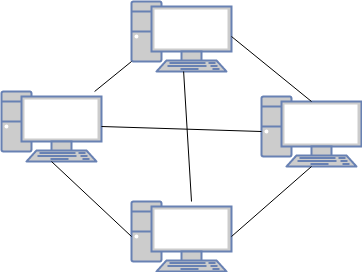
\includegraphics[scale=0.6]{img/Gos}
\caption{Tranzakcijų vėlavimas} % Antraštė įterpiama po paveikslėlio
\label{img:mlp}
\end{figure}

Patvarumas Cassandra duomenų bazėje yra užtikrinamas naudojant patvirtinimų žurnalą kaip sistemos atstatymo mechanizmą. Įrašai nebus pripažinti tinkle kol jie nebus įrašyti į patvirtinimų žurnalą. Po to kai įrašas atsiranda žurnale jis yra perduodamas į vietinę atmintį(memtable) ir kai tų įrašų kiekis pasiekia tam tikra ribą jie yra perkeliami į diską SSTable formatu.
\linebreak
Įrašai Cassandra duomenų bazėje yra labai greiti, nes atliekant rašymo užklauso nėra poreikio atlikti disko skaitymo ir paieškų. Šis funkcionalumas yra pasiekiamas naudojant memtable ir SSTable. Reliacinėse duomenų bazėse atlikti rašymą reikalauja daugiau resursų negu Cassandra duomenų bazėje.

\subsubsection{Testavimo metodologija}
\begin{center}
\begin{tabular}{ | m{5em} | m{10cm}| } 
\hline
\cite{BITCass}& Testai buvo atlikti su trimis HP serveriais DL380
G7 iš viso su 16 branduolių (naudojant HyperThreading) ir 64 GB RAM ir HDD 400
GB. Red Hat Enterprise Linux Server 7.3 (Maipo) (Kernel
Linux 3.10.0-514.e17.x86 64) ir Cassandra 3.11.0 yra įdiegta į visus kompiuterius, taip pat ir virtualias mašinas. Ta pati Cassandra versija naudojama ir apkrovos generavimui. 
Konteinerių testavimui naudota,
Docker versija 1.12.6. Virtualioms mašinoms naudota VMware ESXi 6.0.0.\\ 
\hline
\cite{BITCass}& Testai buvo leidžiami naudojant
Ubuntu Server 12.04 32bit Virtual Machine leidžiant ant VMware Player.
Virtuali mašina turėjo 2GB RAM ir priimančioji mašina turi vieno mazgo Core 2 Quad 2.40
GHz su 4GB RAM ir Windows 7 operacine sistema. Duomenų bazių versijos: MongoDB version 2.4.3
ir Cassandra version 1.2.4. \\ 
\hline
\end{tabular}
\end{center}

\begin{figure}[H]
\centering
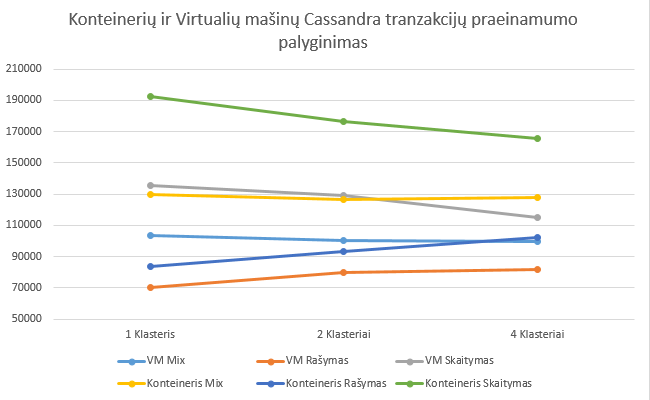
\includegraphics[scale=0.5]{img/CasTh}
\caption{Transakcijų vėlavimas} % Antraštė įterpiama po paveikslėlio
\label{img:mlp}
\end{figure}
\begin{figure}[H]
\centering
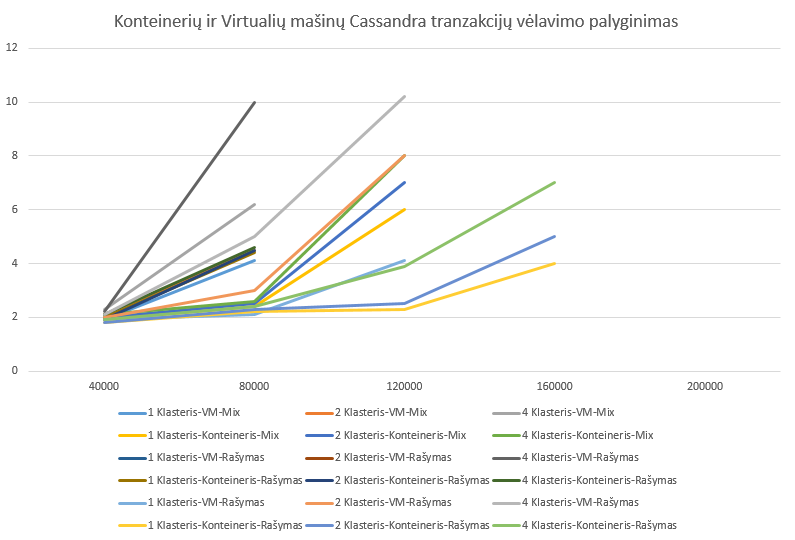
\includegraphics[scale=0.5]{img/CasLat}
\caption{Transakcijų vėlavimas} % Antraštė įterpiama po paveikslėlio
\label{img:mlp}
\end{figure}
\begin{figure}[H]
\centering
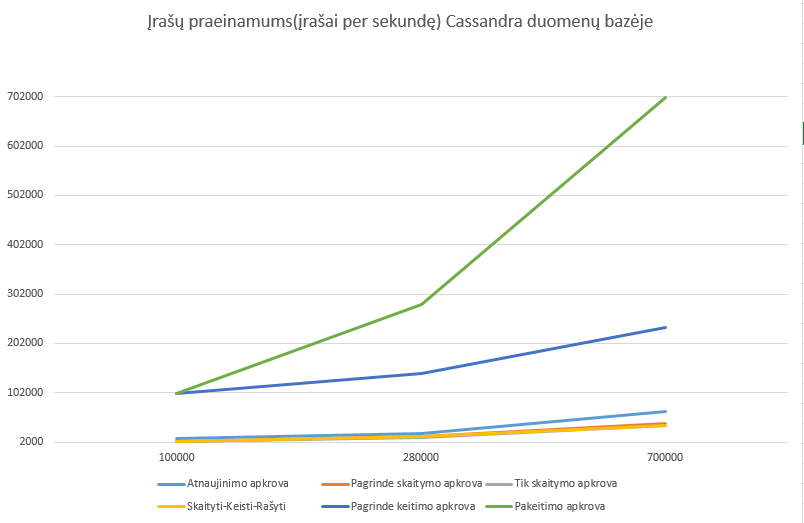
\includegraphics[scale=0.5]{img/CasTp}
\caption{Transakcijų vėlavimas} % Antraštė įterpiama po paveikslėlio
\label{img:mlp}
\end{figure}
\subsubsection{Blekinge technologijų instituto tyrimo rezultatai}
Blekinge technologijų instituto atliktame tyrime \cite{BITCass} buvo atliktas Cassandra duomenų bazės našumo palyginimas lyginant duomenų bazę veikiančia konteineriuose ir virtualioje mašinoje. Buvo lyginama transakcijų praeinamumas ir vėlavimas keičiant klasterių skaičių. Įvairioje apkrovoje virtualios mašinos praeinamumas laikėsi apie 100000 transakcijų per sekundę, rašymo apkrovoje apie 75000 transakcijų per sekundę, skaitymo apkrovoje apie 120000 transakcijų per sekundę.
Įvairioje apkrovoje konteinerių praeinamumas buvo apie 127000 transakcijų per sekundę, rašymo apkrovoje apie 95000 transakcijų per sekundę, o skaitymo apkrovoje apie 180000 transakcijų per sekundę. Virtualiose mašinose didinant klasterių skaičių padidėjo praeinamumas didėjo su rašymo apkrova ir mažėjo su skaitymo apkrova. Tas pats buvo pastebėta ir konteineriuose.
\newline
Tyrime mažiausias vėlavimas buvo naudojant vieną Cassandrą klasterį su 40000 tranzakcijų apkrova, o didžiausias vėlavimas buvo pastebėtas naudojant keturis Cassandra klasterius veikiančius ant virtualių pašinų naudojant 120000 tranzakcijų apkrovą. 
Viso tyrimo metu buvo pastebėtas vėlavimas intervale nuo 1 iki 11 milisekundžių.
\subsubsection{Coimbra politechnikos instituto tyrimo rezultatai.}
Coimbra politechnikos instituto atliktame tyrime \cite{MonCas} buvo lyginamos Cassandra ir MongoDB duomenų bazės. 
Lyginimas buvo atliktas naudojant tik vieną mazgą todėl buvo lygintas tik įrašų(tranzakcijų) praeinamumas su skirtingomis apkrovomis. 
Šio darbo tikslui žiūrėsime tik į rezultatus gautus apie Cassandra duomenų bazę. Pastebėta, kad didinant apkrovą tranzakcijų praeinamumas padidėjo. 
Didžiausias praeinamumas buvo pasiektas kai buvo atlikta tik vieno tipo, o ne miksuotos duomenų operacijos.
Aukšiausias duomenų pakeitimo praeinamumas buvo 700000 tranzakcijų per sekundę, o skaitymo praeinamumas buvo 35000 tranzakcijų per sekundę.
Mažiausias duomenų praeinamumas buvo pastebėtas su mažesnia apkrova.
Žemiausias duomenų pakeitimo praeinamumas buvo 100000 tranzakcijų per sekundę, o žemiausias skaitymo praeinamumas buvo 2325 tranzakcijų per sekundę.
\newline
Pagrindinis šių tyrimų palyginimo trūkumas yra tai, kad visi šiame darbe apžvelgti tyrimai buvo atlikti su skirtingo galingumo sistemomis ir skirtingomis duomenų bazių konfigūracijomis. 
Ieškant literatūros šiam darbui kilo sunkumų surasti tyrimų kuriuose su ta pačia ar panašia kompiuterine įranga ir duomenų bazių konfigūracijomis tiesiogiai būtų lyginamos blokų grandinių duomenų bazės su NoSQL duomenų bazėmis. Sekančiame skirsnyje bus atliekamos Fabric ir Cassandra našumo tyrimas.
\subsection{Greičių tyrimų apibendrinimas}
\begin{figure}[H]
\centering
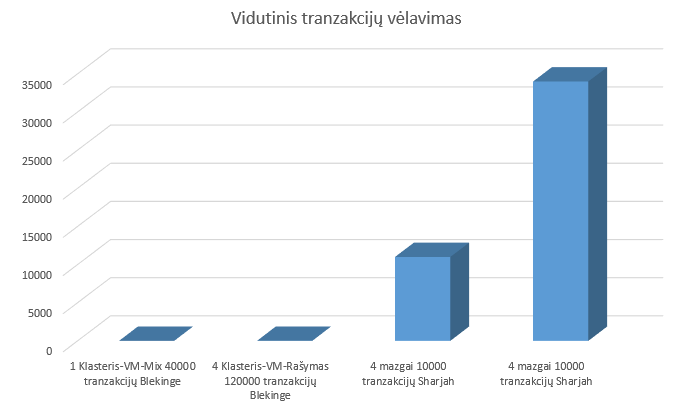
\includegraphics[scale=0.5]{img/CasHypLat}
\caption{Transakcijų vėlavimas} % Antraštė įterpiama po paveikslėlio
\label{img:mlp}
\end{figure}
\begin{figure}[H]
\centering
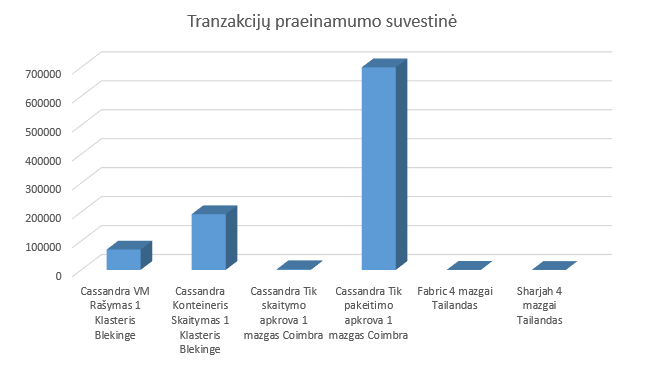
\includegraphics[scale=0.5]{img/CasHypTp}
\caption{Transakcijų vėlavimas} % Antraštė įterpiama po paveikslėlio
\label{img:mlp}
\end{figure}

Apžvelgtuose darbuose buvo matuojamos Apache Cassandra ir Hyperledger Fabric duomenų bazių praeinamumas ir vėlavimas.
Palyginus rezultatus buvo aiškiai matoma, kad Cassandra praeinamumas buvo didesnis ir vėlavimas mažesnis. 
Net ir palyginus prasčiausią Cassandra praeinamumo rezultatą (2325 transakcijų per sekundę) ir geriausią Fabric rezultatą (300 transakcijų per sekundę) Cassandra duomenų bazės praeinamumas buvo geresnis 775 procentais. Lyginant prasčiausią Cassandra ir geriausią Fabric vėlavimo rezultatą Cassandra vėlavimas buvo 1078 procentų mažesnis negu Fabric.
\pagebreak

\section{Duomenų bazių palyginimas pagal CAP teoremą}
\subsection{CAP teorema}
Eric A. Brewer 2000 \cite{CAP} metais pristatė savo teoremą sakančia, kad tinklinis servisas negali užtikrinti trijų savybių vienu metu:
\begin{itemize}
\item{Neprieštaringumas(Consistency) - kiekviena skaitymo užklausa gauna naujausią informaciją arba klaidos pranešimą.}
\item{Pasiekiamumas(Availability) - kiekviena užklauso gauna atsakymą, be garantijos, kad atsakyme bus naujausias įrašas. }
\item{Skaidinių toleravimas(Partition tolerance) - sistema nesustoja funkcionuoti jeigu būna prarandamas arbitrišką skaičių žinučių.}
\end{itemize}
Šios teoremos įrodymas pateikiamas Seth Gilbert ir Nancy Lynch straipsnyje \cite{CAPP}
\linebreak
Kuriant paskirstytąsias sistemas, pagal panaudojimo atvejį, svarbu pasirinkti kuriuos du principus tenkins kuriama paskirstytoji sistema.
Sekančiame skirsnyje bus apžvelgiama Hyperledger Fabric ir Cassandra atitikimas pagal CAP teoremą.
\subsection{Hyperledger Fabric pagal CAP teoremą}
Romos ir Southampton universitetų mokslininkų darbe \cite{BCCAP} buvo tiriama kaip skirtingi susitarimo algoritmai įtakoja Etherium blokų grandinę
pagal CAP teoremą. Šiame darbe CAP buvo pateiktas kitos, labiau blokų grandines atitinkantis CAP teoremos apibrėžimas:
\begin{itemize}
\item{Neprieštaringumas(Consistency) - blokų grandinė yra neprieštaringa, jeigu yra išvengta išsišakojimų. Neprieštaringumas yra pasiekiamas 
susitarimo algoritmų. Jeigu neprieštaringumas nebūna pasiekiamas turime nurodyti, ar jis bus pasiektas vėliau(galiausiai neprieštaringas) ar nebus pasiektas niekada(prieštaringas) }
\item{Pasiekiamumas(Availability) - blokų grandinė yra pasiekiama, jeigu klientų pateiktos transakcijos yra apdorojamos ir galiausiai patvirtinamos ir visam laikui pridedamos prie grandinės}
\item{Skaidinių toleravimas(Partition tolerance) - kai įvyksta tinklo skaidymasis, valdžia yra paskirstoma į atskiras grupes taip, kad skirtingos grupės negali komunikuoti tarpusavyje. Blokų grandinė turi toleruoti 1. Periodus kai tinklas veikia asinchroniškai 2. Atitinkama skaičių Bizantinių valdžių siekiančių sutrikdyti pasiekiamumą ir neprieštaringumą.}
\end{itemize}
Naudojantis šiais CAP apibrėžimais sekančiuose skyriuose bus įvertinta Hyperledger fabric blokų grandinių duomenų bazė.
\subsection{Hyperledger Fabric neprieštaringumas}
Hyperledger Fabric yra vadinamas ,,galiausiai neprieštaringas", nes norint įrašyti transakciją į blokų grandinę užtrunka laiko ją patvirtinti. Klientas sudaro savo transakciją ir išsiunčia ją patvirtinimo perą, patvirtinimo lygiarangis simuliuoja transakcijos pridėjimą į grandinę siekdamas užtikrinti pridėjimo teisingumą. Jeigu simuliacija įvyko sėkmingai tuomet transakciją gauna patvirtinimo parašą ir keliauja atgal pas klientą, kuris išsiunčia jau patvirtiną transakciją į rikiavimo servisą kuris išsiunčia naują grandinės būseną visiems tinklo perams. Per laiko tarpą, kuris praeina nuo kliento transakcijos išsiuntimo patvirtinimo perams iki laiko kol rikiavimo servisas visiems tinklo perams išsiunčia naują grandinės būseną kiti tinklo klientai gali atlikti savo transakcijas nežinodami, kad kiti klientai taip pat darbo transakciją. Duomenų neprieštaringumą užtikrina rikiavimo servisas naudodamas susitarimo algoritmą todėl galiausiai visi tinklo perai gaus atnaujint informaciją, tačiau nebus užtikrinta, kad grandinė kurią gavo lygiarangis yra pačios naujausios versijos. \cite{HypDoc}
\subsection{Hyperledger Fabric pasiekiamumas}
Pasiekiamumą Fabric užtikrina pasiekiamumas laikydama grandinės kopijas visuose peruose, todėl klientas visados galės atlikti transakcijas į blokų grandinę. \cite{HypDoc}
\subsection{Hyperledger Fabric skaidinių toleravimas}
Skaidinių toleravimas yra užtikrintas visą tinklą paskirsčius ant daugelio mazgų. Tinklas išlieka veikiantis, net ir tam tikras mazgų skaičius dingtų, vartotojai vis tiek galėtų siųsti transakcijas į kitus mazgus\cite{HypDoc}.
\subsection{Cassandra neprieštaringumas}
Kai duomenys yra rašomi į duomenų bazę užtrunka laiko duomenys pateks į visus tinklo mazgus. Kai kurie mazgai gali būtų nepasiekiami. Cassandra yra ,,galiausiai neprieštaringa" duomenų baze, nėra užtikrinta, kad duomenys kurie yra skaitomi yra naujausios versijos visame tinkle. 
Cassandra duomenų bazėje yra įgyvendintas pasirenkamasis pasiekiamumas kai klientas pats gali nurodyti kokios lygio neprieštaringumo jis nori skaitant duomenis(mazgų skaičius kurie turi identiškus duomenis) ir rašant duomenis(į kiek mazgų bus įrašyti duomenys). Cassandra duomenų bazėje nėra užtikrinamas neprieštaringumas, nes jeigu kažkuris mazgas yra nepasiekiamas vykdant skaitymą arba rašymą ir jį pasiekti būtina siekiant užtikrinti neprieštaringumą operacija neįvyks. \cite{CasDesk}
\subsection{Cassandra pasiekiamumas}
Rašant duomenis į Cassandra duomenų bazę yra padaromos kelios kopijos ir išsiunčiamos skirtingiems klasterio mazgams. Tai yra užtikrinamas, kad jeigu mazgas tampa nebepasiekiamu duomenys nebūna prarandami.\cite{CasDesk} Duomenų replikavimo lygį galima nurodyti kuriant duomenų bazę. 
\subsection{Cassandra skaidinių toleravimas}
Cassandra duomenų bazė tenkina skaidinių toleravimo principą, nustojus veikti tam tikram skaičiui mazgų tinkle sistemos veikimas nenutrūksta. \cite{CasDesk} 
\subsection{Apibendrinimas}
\begin{figure}[H]
\centering
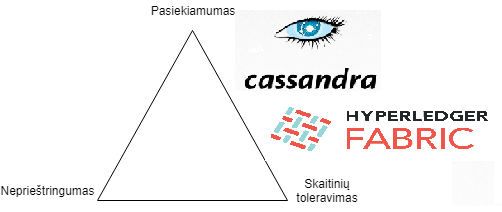
\includegraphics[scale=1]{img/CAP}
\caption{Transakcijų vėlavimas} % Antraštė įterpiama po paveikslėlio
\label{img:mlp}
\end{figure}

Hyperledger Fabric ir Apache Cassandra duomenų bazės įgyvendina pasiekiamumo ir patricijų toleravimo kriterijus CAP teoremoje. Kuriant Cassandra duomenų bazę yra galimybė 
pakeisti konfigūracija taip, kad rašymo operacija būtų laiko sėkminga tik tuomet, kai visiems klasterio mazgams yra padaroma replika, panašiai ir skaitant galima skaityti informacija iš visų tinklo mazgų ir pasirinkti tą informaciją, kuri yra didžiojoje daugumoje mazgų. Pasirinkus tokią konfigūraciją Cassandra labiau pradeda atitikti neprieštaringumo ir patricijų toleravimo savybes tačiau tokia konfigūracija reikalauja paaukoti transakcijų greitį. Hyperledger Fabric nesuteikia tokios konfigūravimo galimybės.

\pagebreak
\section{Rezultatai ir išvados}
\thispagestyle{empty} 
\subsection{Rezultatai}
\begin{enumerate}
\item{Išskirtos dvi bendros metrikos pagal kurias galima palyginti Apache Cassandra ir Hyperledger Fabric : transakcijų }
\item{Aprašytas transakcijų praeinamumo ir vėlavimo priklausomybė nuo mazgų skaičiaus tinkle.}
\item{Išskirti Hyperledger Fabric parametrai kuriuos keičiant keičiasi sistemos veikimo greitis.}
\item{Įvertinta Cassandra ir Hyperledger architektūros atitikimas CAP teoremos principus.}
\end{enumerate}
\subsection{Išvados}
\begin{enumerate}
\item{Yra trūkumas tyrimų lyginančių blokų grandinių duomenų bazių greičius su paskirstytoms duomenų bazės.}
\item{Numatytoji Cassandra ir Hyperledger Fabric duomenų bazių realizaciją, CAP teoremoje, atitinka pasiekiamumo ir skaidymo toleravimo principus.}
\item{Cassandra konfigūracija yra lankstesnė ir leidžia kuriant duomenų bazę padidinti duomenų neprieštaringumą sumažinus transakcijų įvykdymo greitį.}
\item{Cassandra duomebų bazė yra ženkliai greitesnė(iš apžvelgtų straipsnių bent 7 kartus) negu Hyperledger Fabric.}
\end{enumerate}
\subsection{Rekomendacijos ateities darbams}
\begin{enumerate}
\item{Atlikti Cassandra ir Hyperledger Fabric praeinamumo ir vėlavimo tyrimą atlikti naudojant tą pačią kompiuterinę įrangą.}
\item{Atlikti Cassandra praeinamumus ir vėlavimo tyrimą keičiant konfigūraciją link transakcijų neprieštaringumo pusės ir lyginti lėtėjantį greitį su Hyperledger Fabric greičiu.}
\item{Atlinkti greičio lyginimo tyrimus su skirtingomis Fabric ir Cassandra versijomis.}
\end{enumerate}

\pagebreak

\section{Priedai}
\thispagestyle{empty} 
\subsection{Žodynas}
\begin{itemize}

\item{Didžioji knyga(angl. ledger) - transakcijų kaupimo vieta.}
\item{Grandinės kodas(angl. chaincode) - programa parašyta Go, Java arba NodeJS kalbomis kuri vykdo
verslo logiką sutartą tarp tinklo narių.}
\item{Išmanusis kontraktas(angl. smart contract) - kompiuteriu protokolas kurio paskirtis yra  patvirtinti susitarimą.}
\item{Lygiarangis(angl. peer) - tinklo dalyvis gaunantis ir siunčiantis informaciją.}
\item{Mazgas(angl. node) - galutinis taškas arba įrenginys kompiuterių tinkle.}
\item{Paskalos protokolas(angl. gossip protocol) - procedūra kai vieną rangių tinkle informaciją vienas tinklo mazgas perduoda savo kaimynams, o kaimynai savo kaimynams iki tol kol visas tinklas gauna informaciją.}
\item{Skaidymas(angl. partion) - loginės duomenų bazės struktūros padalijimas.}
\item{Transakcija(angl. transaction) - loginis vienetas kuriame yra vienas arba daugiau duomenų perdavimo sakinių.}
\end{itemize}
\thispagestyle{empty} 

\printbibliography[heading=bibintoc] 
\thispagestyle{empty} 
\end{document}

